\section{ХОД РАБОТЫ}

\subsection{Формулировка задачи}

Требуется рассчитать матрицы вероятностей перехода, векторы безусловных вероятностей
и среднее состояние цепи Маркова для последовательности $ n $ шагов,
построить графики изменения значений первой строки матрицы вероятностей перехода,
безусловных вероятностей и среднего состояния.

Исходные данные:
\begin{equation*}
P = \begin{pmatrix}
      0{,}6 & 0 & 0{,}4 \\
      0{,}4 & 0{,}6 & 0 \\
      0{,}4 & 0{,}2 & 0{,}4 \\
    \end{pmatrix},
A = \begin{pmatrix}
      0{,}3 & 0{,}7 & 0
    \end{pmatrix},
E = \begin{pmatrix}
      5 & 6 & 7
    \end{pmatrix}.
\end{equation*}


\subsection{Теоретические сведения}

Рассмотрим переходы системы на протяжении последовательных $ n $ шагов.
Пусть $ P_n $ --- матрица вероятностей перехода за эти $ n $ шагов,
$ P_m $ --- матрица вероятностей перехода за первые $ m $ шагов, $ m < n $,
$ P_{n-m} $ --- матрица вероятностей перехода за оставшиеся $ (n-m) $ шагов.
Тогда выполняется равенство~\ref{eq:Chapman_Kolmogorov_equation}.
\begin{equation}
\label{eq:Chapman_Kolmogorov_equation}
  P_n = P_m P_{n-m}, \hspace{5mm} 0 < m < n.
\end{equation}

Действительно, переход за $ n $ шагов возможен только через одно из состояний
на $ m $-м шаге. Поэтому по формуле полной вероятности получим:
\begin{equation*}
  P_{i,j}(n) = \sum\limits_{\nu}^{\infty} p_{i,\nu}(m) p_{\nu,j}(n-m).
\end{equation*}

\pagebreak

Из уравнения~\ref{eq:Chapman_Kolmogorov_equation} при $ n = 2 $ получим, что
$ P_2 = P_1 P_1 = P_1^2 = P^2 $, при $ n = 3 $ получаем
$ P_3 = P_1 P_2 = P_2 P_1 = P_1^3 = P^3 $. Таким образом для любого $ n $
выполняется равенство~\ref{eq:transition_matrix}.
\begin{equation}
\label{eq:transition_matrix}
  P_n = P^n.
\end{equation}

Абсолютные (безусловные) вероятности состояния системы на $n$-м шаге определяются
выражением~\ref{eq:state_probs}.
\begin{equation}
\label{eq:state_probs}
  a_i(n) = P(\xi_n = E_i), i = 1,2,...
\end{equation}

Такие вероятности определяют вектор-строку безусловных вероятностей $ A_n^T $
системы для момента времени $ n $:
\begin{equation*}
  A_n^T = (a_1(n), a_2(n), ...,) = (a_i(n)), i = 1,2,...
\end{equation*}

Для полного описания однородной цепи Маркова необходимо знать матрицу
вероятностей перехода $P$ и вектор безусловных вероятностей $A_0^T$ для
начального момента времени $ n = 0 $. Этих данных достаточно, чтобы найти
вектор безусловных вероятностей $A_n^T$ для любого $n$ шага с помощью
формулы~\ref{eq:unconditional_probs}.
\begin{equation}
\label{eq:unconditional_probs}
  A_n^T = A_0^T P_n .
\end{equation}

\subsection{Ход работы}

Рассчитаем матрицы вероятностей перехода, векторы безусловных вероятностей
и среднее состояние цепи Маркова для последовательности десяти шагов.

\newpage
Результаты расчёта приведены на рисунке~\ref{lst:results}.
\begin{lstlisting}[caption=Результаты расчётов для десяти шагов,label=lst:results,
basicstyle=\scriptsize\ttfamily]
 PROBABILITY MATRIX #0:                       PROBABILITY MATRIX #1:
 [[ 0.6  0.   0.4]                            [[ 0.52  0.08  0.4 ]
  [ 0.4  0.6  0. ]                             [ 0.48  0.36  0.16]
  [ 0.4  0.2  0.4]]                            [ 0.48  0.2   0.32]]
 STATE PROBABILITIES #0:                      STATE PROBABILITIES #1:
 [ 0.46  0.42  0.12]                          [ 0.492  0.276  0.232]
 AVERAGE STATE: 5.66                          AVERAGE STATE: 5.74

 PROBABILITY MATRIX #2:                       PROBABILITY MATRIX #3:
 [[ 0.504  0.128  0.368]                      [[ 0.5008  0.1504  0.3488]
  [ 0.496  0.248  0.256]                       [ 0.4992  0.2     0.3008]
  [ 0.496  0.184  0.32 ]]                      [ 0.4992  0.1744  0.3264]]
 STATE PROBABILITIES #2:                      STATE PROBABILITIES #3:
 [ 0.4984  0.212   0.2896]                    [ 0.49968  0.18512  0.3152 ]
 AVERAGE STATE: 5.7912                        AVERAGE STATE: 5.81552

 PROBABILITY MATRIX #4:                       PROBABILITY MATRIX #5:
 [[ 0.50016  0.16     0.33984]                [[ 0.500032  0.163968  0.336   ]
  [ 0.49984  0.18016  0.32   ]                 [ 0.499968  0.172096  0.327936]
  [ 0.49984  0.16992  0.33024]]                [ 0.499968  0.168     0.332032]]
 STATE PROBABILITIES #4:                      STATE PROBABILITIES #5:
 [ 0.499936  0.174112  0.325952]              [ 0.4999872  0.1696576  0.3303552]
 AVERAGE STATE: 5.826016                      AVERAGE STATE: 5.830368

 PROBABILITY MATRIX #6:                       PROBABILITY MATRIX #7:
 [[ 0.5000064  0.1655808  0.3344128]          [[ 0.50000128  0.16623104  0.33376768]
  [ 0.4999936  0.1688448  0.3311616]           [ 0.49999872  0.1675392   0.33246208]
  [ 0.4999936  0.1672064  0.3328   ]]          [ 0.49999872  0.16688384  0.33311744]]
 STATE PROBABILITIES #6:                      STATE PROBABILITIES #7:
 [ 0.49999744  0.1678656   0.33213696]        [ 0.49999949  0.16714675  0.33285376]
 AVERAGE STATE: 5.83213952                    AVERAGE STATE: 5.832854272

 PROBABILITY MATRIX #8:
 [[ 0.50000026  0.16649216  0.33350758]
  [ 0.49999974  0.16701594  0.33298432]
  [ 0.49999974  0.16675379  0.33324646]]
 STATE PROBABILITIES #8:
 [ 0.4999999  0.1668588  0.3331413]
 AVERAGE STATE: 5.8331414016

 PROBABILITY MATRIX #9:
 [[ 0.50000005  0.16659681  0.33340314]
  [ 0.49999995  0.16680643  0.33319363]
  [ 0.49999995  0.16670157  0.33329848]]
 STATE PROBABILITIES #9:
 [ 0.49999998  0.16674354  0.33325648]
 AVERAGE STATE: 5.8332564992

 PROBABILITY MATRIX #10:
 [[ 0.50000001  0.16663871  0.33336127]
  [ 0.49999999  0.16672258  0.33327743]
  [ 0.49999999  0.16668064  0.33331937]]
 STATE PROBABILITIES #10:
 [ 0.5         0.16669742  0.33330258]
 AVERAGE STATE: 5.83330258739
\end{lstlisting}

\newpage

Графики изменения значений первой строки матрицы вероятностей перехода,
безусловных вероятностей и среднего состояния цепи Маркова приведены на
рисунках~\ref{pic:hop_probs}~--~\ref{pic:state_probs}.

\begin{figure}[h!]
  \centering
  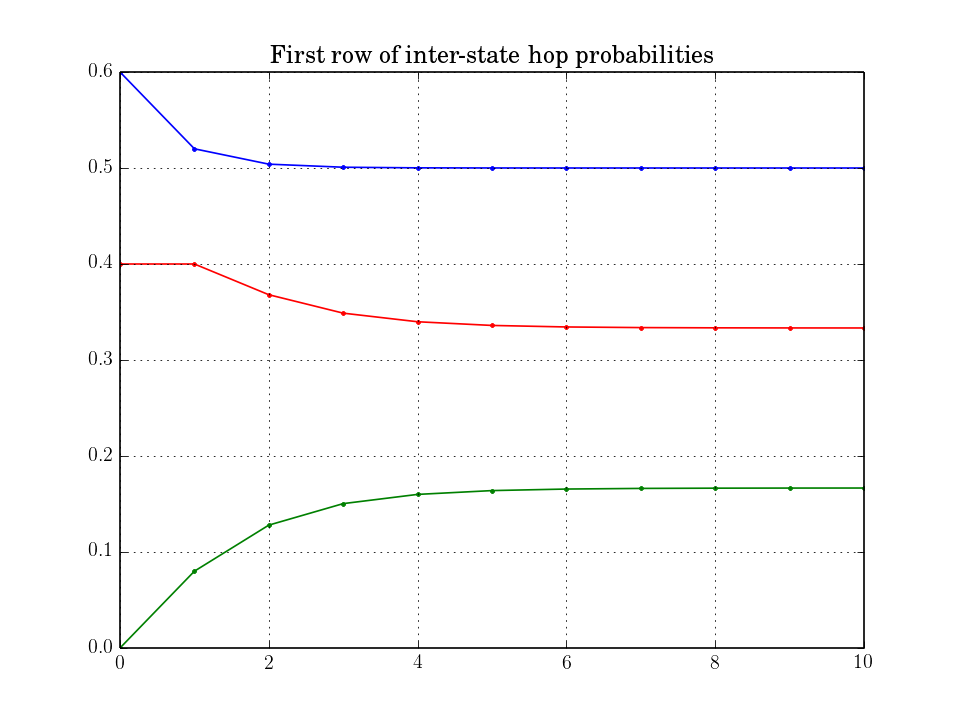
\includegraphics[width=150mm, height=85mm]{pic/hop_probs}
  \caption{Изменение значений первой строки матрицы \\ вероятностей перехода}
  \label{pic:hop_probs}
\end{figure}

\begin{figure}[h!]
  \centering
  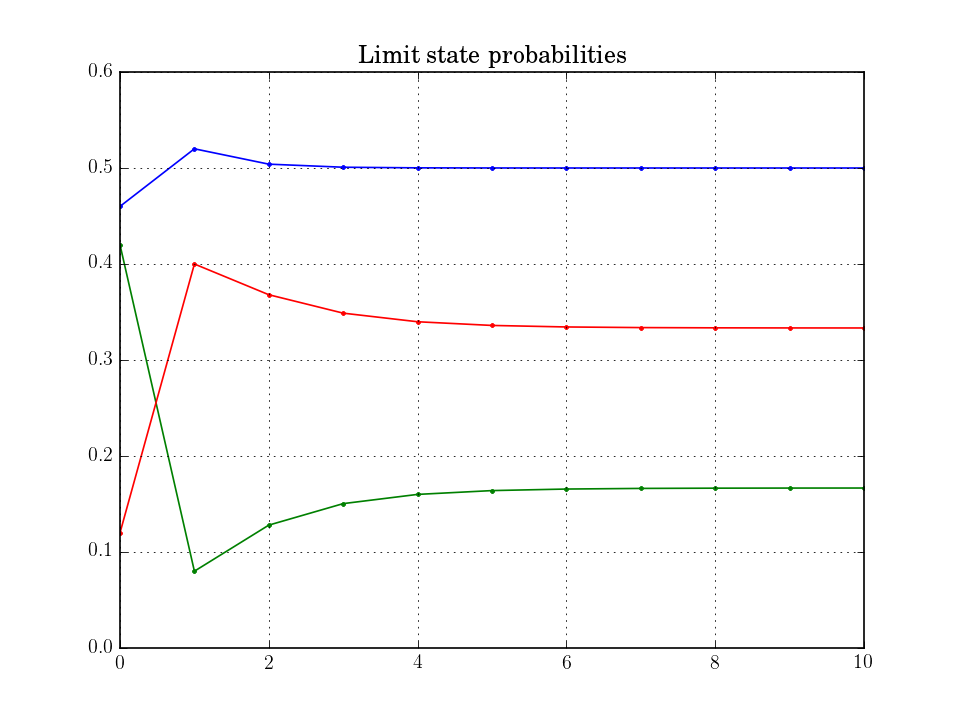
\includegraphics[width=150mm, height=85mm]{pic/state_probs}
  \caption{Изменение значений безусловных вероятностей \\ цепи Маркова}
  \label{pic:state_probs}
\end{figure}

\newpage

\begin{figure}[h!]
  \centering
  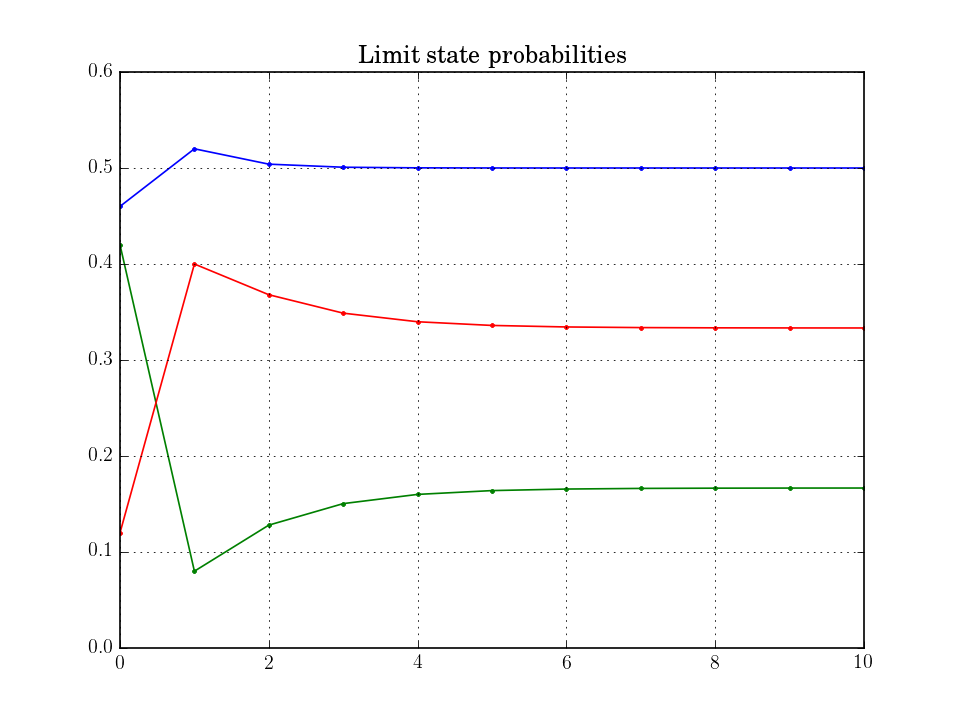
\includegraphics[width=150mm, height=92mm]{pic/state_probs}
  \caption{Изменение среднего состояния цепи Маркова}
  \label{pic:state_probs}
\end{figure}

Исходный код разработанной программы представлен в приложении~А.
